\subsection{Modulation}
\begin{enumerate}[label=\thesubsection.\arabic*.,ref=\thesubsection.\theenumi]

\numberwithin{equation}{enumi}
\numberwithin{figure}{enumi}


\item See Fig. \ref{fig:ee18btech11012_fig1} for the constellation diagram.  The transmitted symbol set is given by 
\begin{align}
\vec{s}_m = \myvec{\cos \frac{2m\pi}{8}\\ \sin \frac{2m\pi}{8}}, \quad m \in \cbrak{0,1,\dots,7}.
%\textbf{y = s + n}
\end{align}
%
The numerical values for $\vec{s}_m$ are listed in Table \ref{table: }
\begin{figure}[!ht]
                \resizebox{\columnwidth}{!}{\input{./ee18btech11012/figs/8psk_constellation.tex}}
\label{fig:ee18btech11012_fig1}
\caption{Constellation diagram}
\end{figure}


\item The gray code shown in Table \ref{table: } is used for encoding the 8-PSK symbols.

%$s_0$ denote bits 000, $s_1$ denote bits 001, $s_2$ denote bits 011,$s_3$ denote bits 010,$s_4$ denote bits 110,$s_5$ denote bits 111,$s_6$ denote bits 101,$s_7$ denote bits 100.

\item The received symbol is then obtained as
\begin{align}
\vec{y} = \sqrt{E_s}\vec{s} + \vec{n}
\end{align}
%
where $E_s$ is the symbol energy and 

\begin{align}
\vec{n} &\sim \mathcal{N}\brak{\vec{0},\frac{N_0}{2}\vec{I}}
\\
\vec{s} &\in \cbrak{\vec{s}_m}_{m = 0}^{7}
\end{align}

\item The decision rule is given by Fig. \ref{fig:ee18btech11012_fig2} and can be expressed as



\begin{figure}[!ht]

                \resizebox{\columnwidth}{!}{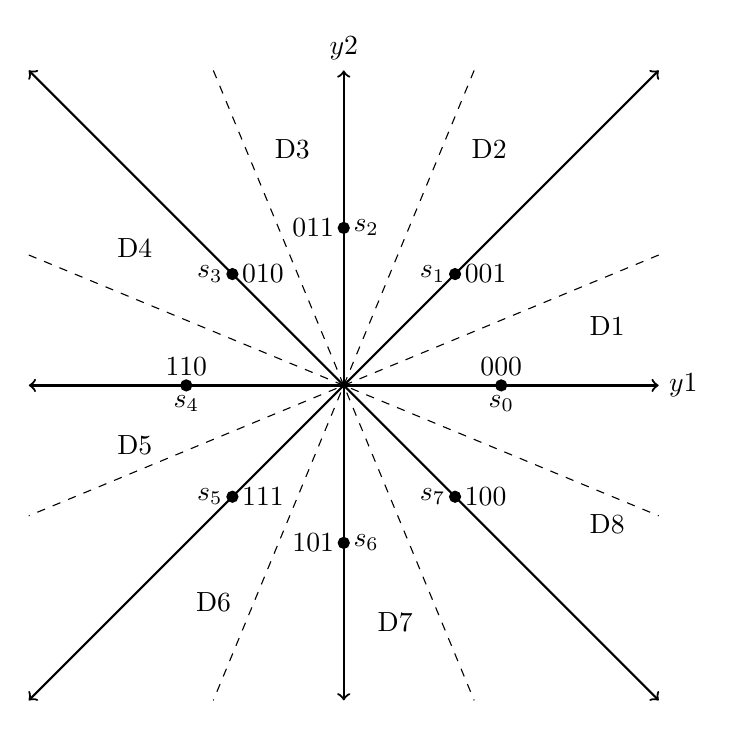
\begin{tikzpicture}

\draw[<->,thick] (-4,0)--(4,0) node[right]{$y1$};
\draw[<->,thick] (0,-4)--(0,4) node[above]{$y2$};
\draw[dashed] (4,1.656)--(-4,-1.656);
\draw[dashed] (1.656,4)--(-1.656,-4);
\draw[dashed] (-1.656,4)--(1.656,-4);
\draw[dashed] (-4,1.656)--(4,-1.656);
\draw[<->,thick](-4,-4)--(4,4);
\draw[<->,thick](-4,4)--(4,-4);

\filldraw[black] (2,0) circle (2pt) node[below] {$s_0$} node[above] {000};
\filldraw[black] (1.414,1.414) circle (2pt) node[left] {$s_1$} node[right] {001};
\filldraw[black] (0,2) circle (2pt) node[right] {$s_2$} node[left] {011};
\filldraw[black] (-1.414,1.414) circle (2pt) node[left] {$s_3$} node [right] {010};
\filldraw[black] (-2,0) circle (2pt) node[below] {$s_4$} node[above] {110};
\filldraw[black] (-1.414,-1.414) circle (2pt) node[left] {$s_5$} node[right] {111};
\filldraw[black] (0,-2) circle (2pt) node[right] {$s_6$} node[left] {101};
\filldraw[black] (1.414,-1.414) circle (2pt) node[left] {$s_7$} node [right] {100};

\foreach \coordinate/\label/\pos in {{(3,1)/D1/below right},{(1.5,3)/D2/right},{(-1,3)/D3/right},{(-3,1.5)/D4/above right},{(-3,-1)/D5/above right},{(-2,-3)/D6/above right},{(1,-3)/D7/left},{(3,-2)/D8/above right}} \node[\pos] at \coordinate {\label};

\end{tikzpicture}
}

\label{fig:ee18btech11012_fig2}
\caption{decision regions}
	
\end{figure}





Let \textbf{r} be the received bits, \textbf{r} = [$r_1$,$r_2$,$r_3$]. 
\begin{align}
    r_1 = 
    \begin{cases}
    0, &  \textbf{y} \in D1\cup D2\cup D3\cup D4 \Leftrightarrow  y_1(\sqrt{2}-1)+y_2>0\\
    1, &  \textbf{y} \in D5\cup D6\cup D7\cup D8 \Leftrightarrow y_1(\sqrt{2}-1)+y_2<0
    \end{cases}
    \label{eq:ee18btech11012_eq1}
\end{align}
\begin{align}
    r_2 = 
    \begin{cases}
    0, &  \textbf{y} \in D2\cup D1\cup D8\cup D7 \Longleftrightarrow  y_2 -(\sqrt{2}+1)y_1<0\\
    1, &  \textbf{y} \in D3\cup D4\cup D5\cup D6 \Longleftrightarrow  y_2 -(\sqrt{2}+1) y_1 > 0
    \end{cases}
    \label{eq:ee18btech11012_eq2}
\end{align}
\begin{align}
    r_3 = 
    \begin{cases}
    0, &  \textbf{y} \in D4\cup D5\cup D1\cup D8 \Longleftrightarrow  y_2 +(\sqrt{2}+1)y_1 < 0 ,  y_2 -(\sqrt{2}-1)y_1 > 0  \\
    1, &  \textbf{y} \in D2\cup D3\cup D6\cup D7 \Longleftrightarrow  y_2 +(\sqrt{2}+1)y_1 > 0 ,  y_2 -(\sqrt{2}-1)y_1 < 0 
    \end{cases}
    \label{eq:ee18btech11012_eq3}
\end{align}

From eq.\ref{eq:ee18btech11012_eq1},eq.\ref{eq:ee18btech11012_eq2} and eq.\ref{eq:ee18btech11012_eq3}
\\
For detecting $s_0$, $y_2+(\sqrt{2}-1)y_1>0$ and $y_2-(\sqrt{2}-1)y_1<0$.
\\
For detecting $s_1$, $y_2-(\sqrt{2}+1)y_1<0$ and $y_2-(\sqrt{2}-1)y_1>0$.
\\
For detecting $s_2$, $y_2-(\sqrt{2}+1)y_1>0$ and $y_2+(\sqrt{2}+1)y_1>0$.
\\
For detecting $s_3$, $y_2+(\sqrt{2}-1)y_1>0$ and $y_2+(\sqrt{2}+1)y_1<0$.
\\
For detecting $s_4$, $y_2+(\sqrt{2}-1)y_1<0$ and $y_2-(\sqrt{2}-1)y_1>0$.
\\
For detecting $s_5$, $y_2-(\sqrt{2}+1)y_1>0$ and $y_2-(\sqrt{2}-1)y_1<0$.
\\
For detecting $s_6$, $y_2-(\sqrt{2}+1)y_1<0$ and $y_2+(\sqrt{2}+1)y_1<0$.
\\
For detecting $s_7$, $y_2+(\sqrt{2}-1)y_1<0$ and $y_2+(\sqrt{2}+1)y_1>0$.




\item The following code has simulation of 8PSK.
\begin{lstlisting}
 codes/8psk.py
\end{lstlisting}




















\end{enumerate}
